
\chapter{Introducción}
En esta memoria se recoge el trabajo  realizado para la solución de las diferentes prácticas de la asignatura, donde	en cada capítulo se recoge la solución de cada práctica y sus diferentes apartados.\\

El primer paso para realización de las prácticas ha sido el montaje del robot, quedando como se muestra en la Figura~\ref{robot}. A medida que sean necesarios diferentes sensores para la realización de las practicas se irán añadiendo.
 
	\begin{figure}[H]
 \centering
 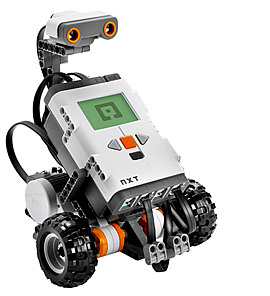
\includegraphics[scale=0.6]{./img/robot.jpg}
 \caption{Lego Mindstorms}
 \label{robot}
\end{figure}

En las prácticas se ha utilizado el lenguaje de implementación de \textbf{OSEK} \cite{NXTweb}.

\chapter{Práctica 1. Manejo básico de Lego Mindstorms NXT: Sensores y Actuadores}


\section{Objetivos}

Tras la realización de esta práctica el alumno debería ser capaz de:
\begin{itemize}
	\item Programar movimientos sincronizados del robot. 
	\item Conocer los parámetros de funcionamiento básico de los motores. 
	\item Utilización  de los sensores básicos. 
\end{itemize}

\section{Ejercicio A}
Calibrar la potencia relativa de los motores para realizar un movimiento lineal con un error menor a 1cm. de desvío por cada 1 m. de avance lineal. (Error menor al 1\%).

\subsection{Estrategia}
El objetivo de este apartado es que el robot avance de manera lineal, sin que se produzcan desviaciones en su trayectoria. \\

Para ello se decide establecer la velocidad de los motores al 50\%, y que este corrija mediante una tarea denominada \textit{calibrar} la velocidad de cada motor, para conseguir un momento lineal sin desviaciones.


\subsection{Tareas}
A continuación se realiza una descripción de las tareas utilizadas para la resolución de este apartado y su prioridad.

\begin{itemize}
	\item \textbf{Avanzar}
		\begin{itemize}
			\item \textit{Prioridad}: 1
			\item \textit{Descripción}: Se ejecuta durante 6000 milisegundos, que es el tiempo que corresponde aproximadamente al avance de un metro. Los motores se activan a una velocidad del 50\%.
		\end{itemize}
	
	\item \textbf{Calibrar}
		\begin{itemize}
			\item \textit{Prioridad}: 2
			\item \textit{Descripción}: Se encarga de calibrar los motores con el fin de que el robot avance recto, esta asociada a la alarma \textit{alarm1}. Pueden ocurrir dos casos:
			\begin{enumerate}
				\item El motor C vaya a más revoluciones que el motor B, entonces para ello se comprueba que la velocidad de este último sea menor que la velocidad establecida al principio (con un margen de más 5), si se cumple se aumenta la velocidad del motor B, en el caso contrario se disminuye la velocidad del motor C.
				\item El caso contrario, que el motor B vaya a más revoluciones que el motor C, entonces se comprueba la velocidad que la velocidad de éste sea menor que la establecida al principio (con un margen de más 5), si se cumple se aumenta la velocidad del motor C, en en caso contrario se disminuye la velocidad del motor B.
			\end{enumerate}
		\end{itemize}
	
	\item \textbf{Final}
		\begin{itemize}
			\item \textit{Prioridad}: 3
			\item \textit{Descripción}: Esta tarea hace detener el robot.
		\end{itemize}
\end{itemize}


En la Figura~\ref{grafico1a}, se muestra un gráfico de su funcionamiento.

\begin{figure}[H]
 \centering
 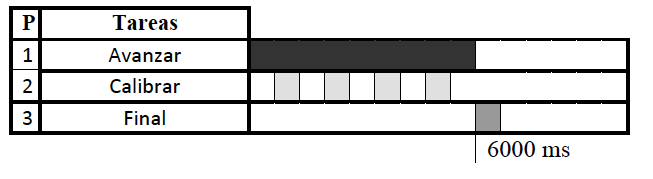
\includegraphics[scale=0.4]{./img/grafico1a.png}
 \caption{Funcionamiento práctica 1a.}
 \label{grafico1a}
\end{figure}

\subsection{Alarmas}
Para la resolución de éste apartado ha sido necesaria la utilización de una alarma.

\begin{itemize}
	\item \textbf{Alarm1}
		\begin{itemize}
			\item \textit{Periodo}: 500 ciclos
			\item \textit{Autoinicio}: Sí
			\item \textit{Descripción}: Esta alarma se encarga de ejecutar la tarea \textit{calibrar} para que se produzca una corrección en los motores si fuese necesario.
		\end{itemize}
			
\end{itemize}
\subsection{Código del fichero practica1\_a.c}
\lstinputlisting{practicas/practica1a/practica_1a.c}


\subsection{Código del fichero practica1\_a.oil}
En este fichero se definen los valores por defecto con los que empieza la ejecución de cada tarea, prioridad, tipo de esquema, si debe iniciarse la tarea al encender el robot o no, etc.

\lstinputlisting{practicas/practica1a/practica_1a.oil}

\subsection{Resultados}
En un principio se pensó realizar la práctica intentado poner a cada motor una potencia para que se produjera el movimiento lineal pero aún así se producía bastante desviación. Finalmente se decidió añadir una alarma que se encargara de calibrar los motores en el movimiento de avance, obteniendo con ello mejores resultados.\\

\textbf{Vídeo}:  \url{http://www.youtube.com/watch?v=tBR9gWx_GH8}
\section{Ejercicio B}

\par Programar una maniobra de aparcamiento del robot sin tener en cuenta sensores. Se muestra una descripción del entorno de aparcamiento (Figura~\ref{aparcamiento}). El robot se posicionará con las ruedas motrices rozando la línea lateral y con las ruedas justo por delante de la línea de inicio.

\begin{figure}[ht!]
 \centering
 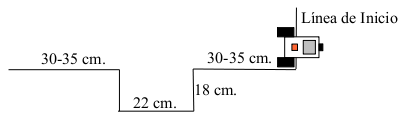
\includegraphics[scale=0.7]{./img/recorrido1.png}
 \caption{Diagrama del aparcamiento.}
 \label{aparcamiento}
\end{figure}

\subsection{Estrategia}
Como se describe en el enunciado se debe realizar la maniobra de aparcamiento sin tener en cuenta los sensores. Nuestra idea a sido simular el aparcamiento igual que sucede con los coches. Para ello se ha establecido el siguiente orden de movimiento:
\begin{enumerate}
	\item Avanzar desde la linea de inicio hasta el punto 1, como se muestra en la Figura~\ref{paso1}.

\begin{figure}[H]
 \centering
 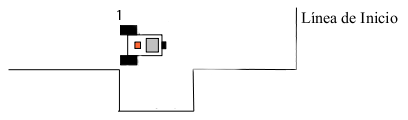
\includegraphics[scale=0.7]{./img/recorrido2.png}
 \caption{Diagrama del aparcamiento - Paso 1.}
 \label{paso1}
\end{figure}

	\item Girar a la derecha hacia atrás, hasta quedar en la posición que se muestra en la  Figura~\ref{paso2}.
	
	\begin{figure}[H]
 \centering
 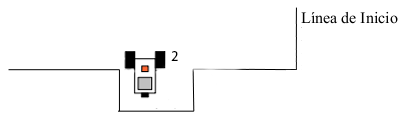
\includegraphics[scale=0.7]{./img/recorrido3.png}
 \caption{Diagrama del aparcamiento - Paso 2.}
 \label{paso2}
\end{figure}

\item Girar a la izquierda hacia atrás, hasta quedar en la posición que se muestra en la  Figura~\ref{paso3}.
	
	\begin{figure}[H]
 \centering
 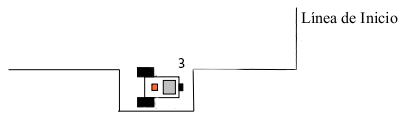
\includegraphics[scale=0.7]{./img/recorrido4.png}
 \caption{Diagrama del aparcamiento - Paso 3.}
 \label{paso3}
\end{figure}

\end{enumerate}

Para saber la distancia que se debe recorrer se calcula el numero de grados que se deben recorrer en cada momento, para ello se ha utilizado la siguiente fórmula:

$$ g=\frac{360  \cdot  d}{2 \cdot \pi \cdot r } $$

donde, \textit{g} es el número de grados recorridos, \textit{d} es la distancia que se quiere recorrer y \textit{r} es el radio de las ruedas.
\subsection{Tareas}
A continuación se realiza una descripción de las tareas utilizadas para la resolución de este apartado y su prioridad.

\begin{itemize}

		\item \textbf{Principal}
		\begin{itemize}
			\item \textit{Prioridad}: 1
			\item \textit{Descripción}: Se encarga de activar las tareas \textit{Avance}, \textit{GiroIzq}, \textit{Retroceso}, \textit{GiroIzq}.
		\end{itemize}
		
		\item \textbf{GiroIzq}
		\begin{itemize}
			\item \textit{Prioridad}: 2
			\item \textit{Descripción}: Se encarga de realizar un giro hacia la izquierda hacia atrás, activando sólo para ello el motor C. Se ejecuta hasta que se realice el giro, ya que con la fórmula se ha calculado cuanto distancia debe durar.
		\end{itemize}
		
		\item \textbf{Retroceso}
		\begin{itemize}
			\item \textit{Prioridad}: 3
			\item \textit{Descripción}: Se encarga de retroceder para ello se activan ambos motores con velocidad negativa. Se ejecuta hasta que se realice el retroceso, ya que con la fórmula se ha calculado.
		\end{itemize}
		
		\item \textbf{GiroDer}
		\begin{itemize}
			\item \textit{Prioridad}: 4
			\item \textit{Descripción}: Se encarga de realizar un giro hacia la derecha hacia atrás, activando sólo para ello el motor B. Se ejecuta hasta que se realice el giro, ya que con la fórmula se ha calculado cuanto distancia debe durar.
		\end{itemize}
		
		
	\item \textbf{Avance}
		\begin{itemize}
			\item \textit{Prioridad}: 5
			\item \textit{Descripción}: Se ejecuta durante el tiempo que tarda en recorrer el la distancia que se ha calculado mediante la fórmula. Se encarga de realizar un avance lineal.
		\end{itemize}
	
	\item \textbf{Calibrar}
		\begin{itemize}
			\item \textit{Prioridad}: 6
			\item \textit{Descripción}: Se encarga de calibrar los motores con el fin de que el robot avance recto, se activa mediante una alarma. Pueden ocurrir dos casos:
			\begin{enumerate}
				\item El motor C vaya a más revoluciones que el motor B, entonces para ello se comprueba que la velocidad de este último sea menor que la velocidad establecida al principio (con un margen de más 5), si se cumple se aumenta la velocidad del motor B, en el caso contrario se disminuye la velocidad del motor C.
				\item El caso contrario, que el motor B vaya a más revoluciones que el motor C, entonces se comprueba la velocidad que la velocidad de éste sea menor que la establecida al principio (con un margen de más 5), si se cumple se aumenta la velocidad del motor C, en en caso contrario se disminuye la velocidad del motor B.
			\end{enumerate}
		\end{itemize}
	
	\item \textbf{Final}
		\begin{itemize}
			\item \textit{Prioridad}: 7
			\item \textit{Descripción}: Esta tarea hace detener el robot.
		\end{itemize}
\end{itemize}


En la siguiente Figura~\ref{grafico1b}, se muestra un gráfico de su funcionamiento.

\begin{figure}[H]
 \centering
 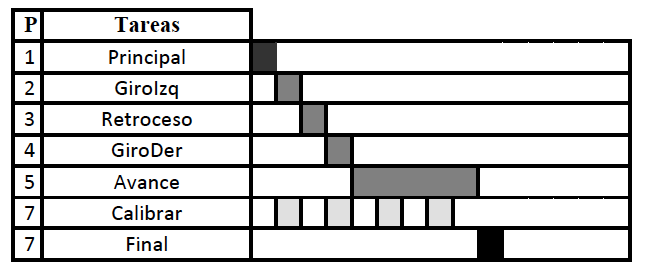
\includegraphics[scale=0.4]{./img/grafico1b.png}
 \caption{Funcionamiento práctica 1b.}
 \label{grafico1b}
\end{figure}

\subsection{Alarmas}
Para la resolución de éste apartado ha sido necesaria la utilización de una alarma.

\begin{itemize}
	\item \textbf{Alarma1}
		\begin{itemize}
			\item \textit{Periodo}: 10 ciclos
			\item \textit{Autoinicio}: Sí
			\item \textit{Descripción}: Esta alarma se encarga de ejecutar la tarea \textit{calibrar} para que se produzca una corrección en los motores si fuese necesario.
		\end{itemize}
			
\end{itemize}

\subsection{Código del fichero practica1\_b.c}
\lstinputlisting{practicas/practica1b/practica_1b.c}

\subsection{Código del fichero practica1\_b.oil}
\lstinputlisting{practicas/practica1b/practica_1b.oil}

\subsection{Resultados}
En el siguiente vídeo se puede observar como resuelve el problema de este apartado, destacar que se ha añadido también la alarma que tiene asociada la tarea calibrar para que el avance sea totalmente recto.\\

\textbf{Video}: \url{http://www.youtube.com/watch?v=N9PUJD5SiOQ}

\section{Ejercicio C}

\par Realizar un movimiento de avance del robot teniendo en cuenta los sensores de ultrasonidos y de pulsación, 
que estarán colocados en el frontal de avance del robot. El robot avanzará a plena potencia hasta que se encuentre 
a 1 m. de un obstáculo, que reducirá su potencia a la mitad. A 20 cm. de distancia del obstáculo, el robot reducirá 
su potencia de avance a un cuarto. El avance continuará hasta que el choque sea detectado por el sensor de pulsación, 
en cuyo caso, el robot retrocederá durante 1 seg. y girará 90º a la derecha, comenzando de nuevo el mismo procedimiento.

\subsection{Estrategia}
Como se indica en el enunciado, el robot debe avanzar a máxima velocidad, para ello hemos decidido definir la tarea avance la cual activará los motores del robot a máxima velocidad. \\

Mediante una alarma asociada a la tarea comprobar, como su nombre indica, se encargará de comprobar la distancia a la que se encuentran los obstáculos con el sensor de ultrasonidos, si esta distancia es menor de \textit{1 m} se reducirá la potencia a la mitad, cuando la distancia sea inferior a \textit{20 cm} se reducirá la potencia a un cuarto, en el momento que se produzca un choque, el cual se comprobará con el sensor de pulsación, se activará la tarea retroceder, esta tarea hará que el robot retroceda durante \textit{1 seg.} y seguidamente se activará la tarea girar a la derecha. Una vez se produce el giro a la derecha se vuelve a activar la tarea avanzar de nuevo.
\subsection{Tareas}
A continuación se realiza una descripción de las tareas utilizadas para la resolución de este apartado y su prioridad.

\begin{itemize}
	
	\item \textbf{Principal}
		\begin{itemize}
			\item \textit{Prioridad}: 1
			\item \textit{Descripción}: Se encarga de activar la tarea \textit{Avance}.
		\end{itemize}

	\item \textbf{Avance}
		\begin{itemize}
			\item \textit{Prioridad}: 2
			\item \textit{Descripción}: Se encarga de activar los motores a una velocidad del 100\%. Se ejecuta mientras no se active una tarea mayor prioridad. 
		\end{itemize}
		
	\item \textbf{Mitad\_Potencia}
		\begin{itemize}
			\item \textit{Prioridad}: 4
			\item \textit{Descripción}: Se encarga de reducir los motores a la mitad de potencia.
		\end{itemize}

	\item \textbf{Cuarto\_Potencia}
		\begin{itemize}
			\item \textit{Prioridad}: 5
			\item \textit{Descripción}: Se encarga de reducir los motores a un cuarto de potencia.
		\end{itemize}	
		
		\item \textbf{Retroceso}
		\begin{itemize}
			\item \textit{Prioridad}: 6
			\item \textit{Descripción}: Se encarga de retroceder durante un segundo y activar la tarea \textit{Giro\_Dcha}.
		\end{itemize}
		
		
		\item \textbf{Giro\_Dcha}
		\begin{itemize}
			\item \textit{Prioridad}: 7
			\item \textit{Descripción}: Se encarga de realizar el giro a la derecha, para ello sólo el motor C.
		\end{itemize}
				
		\item \textbf{Comprueba\_Distancia}
		\begin{itemize}
			\item \textit{Prioridad}: 10
			\item \textit{Descripción}: Tarea asociada a la alarma \textit{alarm1}, la cual se encarga de comprobar la distancia a la que se encuentra un obstáculo, para ello realiza seis medidas a través del sensor de ultrasonidos y calcula la media, en función de la distancia a la que se encuentre el obstáculo se activarán diferentes tareas.
			\begin{enumerate}
				\item Si se encuentra entre una distancia menor de \textit{1 metro} y superior a \textit{20 cm}, se activa la tarea \textit{Mitad\_Potencia} reduciendo la velocidad del robot a la mitad.
				\item Si se encuentra a una distancia inferior a \textit{20 cm}, se activa la tarea \textit{Cuarto\_Potencia} y la velocidad del robot se reduce a un cuarto.
			\end{enumerate}
			
			Si el cualquier momento se activa el sensor de pulsación, esto producirá que se active la tarea \textit{retroceso}.
				
			\end{itemize}
		
\end{itemize}

En la Figura~\ref{grafico1c}, se muestra un ejemplo donde el robot se encuentra un obstáculo:

\begin{figure}[H]
 \centering
 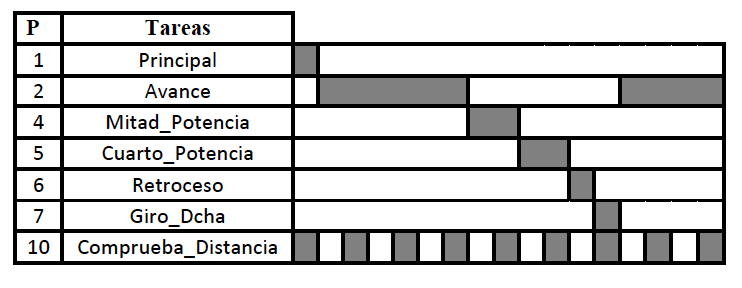
\includegraphics[scale=0.4]{./img/grafico1c.png}
 \caption{Funcionamiento práctica 1c.}
 \label{grafico1c}
\end{figure}

\subsection{Alarmas}
Para la resolución de éste apartado ha sido necesaria la utilización de una alarma.

\begin{itemize}
	\item \textbf{Alarm1}
		\begin{itemize}
			\item \textit{Periodo}: 200 ciclos
			\item \textit{Autoinicio}: Sí
			\item \textit{Descripción}: Esta alarma se encarga de ejecutar la tarea \textit{Comprueba\_Distancia} la cual se encarga de calcular la distancia a la que se encuentran los obstáculos y activar diferentes tareas en función de la distancia que se encuentre el obstáculo.
		\end{itemize}
\end{itemize}
\subsection{Código del fichero practica1\_c.c}
\lstinputlisting{practicas/practica1c/practica_1c.c}

\subsection{Código del fichero practica1\_c.oil}
\lstinputlisting{practicas/practica1c/practica_1c.c}

\subsection{Resultados}
En el siguiente vídeo se muestra el resultado de la práctica.\\

\textbf{Vídeo}:  \url{http://www.youtube.com/watch?v=YRg_E0FvMig}

\chapter{Práctica 2. Manejo básico de Lego Mindstorms NXT: Tareas y Comunicaciones}

\section{Objetivos}
Tras la realización de esta práctica el alumno debería ser capaz de:
\begin{itemize}
	\item Acceder a sensores de manera efectiva.
	\item Realizar programación concurrente con memoria compartida
	\item Realizar comunicaciones distribuidas mediante el modelo cliente-servidor.
\end{itemize}


\section{Ejercicio A}
Construir y programar un robot con un sensor de ultrasonidos que sea capaz de encontrar la salida de un ``laberinto'' (Dicho laberinto será una concatenación de pequeñas estancias rectangulares con una única entrada y una única salida, como puede observarse en la Figura~\ref{laberinto}). 
Se incorporará un sensor de pulsación en la parte superior para indicarle al robot que ha salido del laberinto.

\begin{figure}[H]
 \centering
 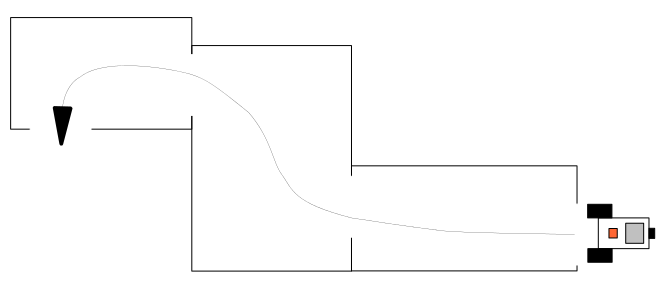
\includegraphics[scale=0.5]{./img/laberinto.png}
 \caption{Diagrama del laberinto.}
 \label{laberinto}
\end{figure}
\subsection{Estrategia}
Para resolución de este apartado ha sido necesario añadir al robot el sensor de utrasonidos para encontrar la salida del laberinto y dos sensores de pulsación, uno delantero para detectar que se ha producido un choque con alguna de las paredes del laberinto y otro superior para indicar al robot que se ha salido del laberinto.\\

La solución propuesta para salir del laberinto ha sido la siguiente, una tarea principal la cual se encarga de avanzar mientras no se produzca choque o se pulse el pulsador de fin de laberinto, si se produce el choque con alguna pared del laberinto retrocederá y activará la tarea giro que se encargará de girar el robot 90 grados hacia la izquierda y derecha y en cada giro medir la distancia, el robot elegirá el camino en el que la distancia sea mayor. \\

También se tendrá una tarea pulsador asociada a una alarma, encargada de comprobar si se ha pulsado el sensor de fin de laberinto.

\subsection{Tareas}

A continuación se realiza una descripción de las tareas utilizadas para la resolución de este apartado y su prioridad.

\begin{itemize}
	
	\item \textbf{Principal}
		\begin{itemize}
			\item \textit{Prioridad}: 1
			\item \textit{Descripción}: Tarea que se ejecuta mientra la bandera fin se encuentre desactivada, es decir mientras no se pulse el pulsador de fin de laberinto. Esta tarea se encargará de que el robot avance, en el momento que se produzca un choque con algunas de las paredes del laberinto el robot retrocederá y activará la tarea \textit{giro}.
		\end{itemize}
		
		\item \textbf{Giro}
		\begin{itemize}
			\item \textit{Prioridad}: 2
			\item \textit{Descripción}: La tarea \textit{giro} se encargará de:
			\begin{enumerate}
				\item Girar el robot \textit{90 grados} hacia la derecha y realizar 10 mediciones con el sensor de ultrasonidos y calcular la distancia media.
				\item Girar el robot \textit{90 grados} hacia la izquierda y realizar 10 mediciones con el sensor de ultrasonidos y calcular al distancia media.
			\end{enumerate}
			
			Una vez realizada las mediciones a ambos lados, el robot comprueba si la distancia a la derecha es mayor que a la izquierda, si es cierto, se vuelve a girar el robot hacia la derecha, en caso contrario, no se gira ya que se encuentra en la mejor dirección.
		\end{itemize}
		
		\item \textbf{Pulsador}
		\begin{itemize}
			\item \textit{Prioridad}: 3
			\item \textit{Descripción}: Tarea asociada a la alarma \textit{alarm1}, la cual se encargará de comprobar que se ha pulsado el sensor fin de laberinto y pondrá la bandera fin a 1 para que la tarea \textit{principal} finalice.
		\end{itemize}
			
\end{itemize}

En la Figura~\ref{grafico2a}, se muestra un ejemplo donde el robot intenta salir del laberinto:

\begin{figure}[H]
 \centering
 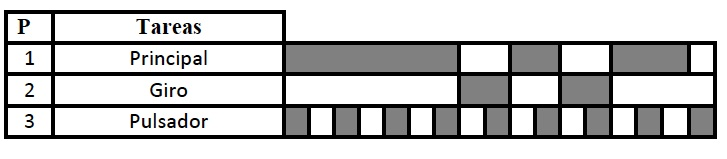
\includegraphics[scale=0.5]{./img/grafico2a.jpg}
 \caption{Funcionamiento práctica 2a.}
 \label{grafico2a}
\end{figure}

\subsection{Alarmas}
\begin{itemize}
	\item \textbf{Alarm1}
		\begin{itemize}
			\item \textit{Periodo}: 100 ciclos
			\item \textit{Autoinicio}: Sí
			\item \textit{Descripción}: Esta alarma se encarga de ejecutar la tarea \textit{Pulsador} la cual se encarga de comprobar de detectar que se ha pulsado el pulsador fin de laberinto.
		\end{itemize}
\end{itemize}
\subsection{Código del fichero practica2\_a.c}
\lstinputlisting{practicas/practica2a/practica_2a.c}

\subsection{Código del fichero practica2\_a.oil}
\lstinputlisting{practicas/practica2a/practica_2a.oil}

\subsection{Resultados}

\section{Ejercicio B}
Programar un segundo robot sin sensores (se podrá utilizar el robot básico de algún compañero), de tal forma que el robot con sensores le envíe mediante comunicaciones bluetooth las órdenes necesarias 
para que el robot sin sensores sea capaz de realizar el recorrido de salida del laberinto. Se recomienda que el robot con sensores almacene todos los datos necesarios y los envíe mediante un modelo cliente-servidor. A su vez, el robot sin sensores debería ejecutar una tras otra las acciones que le ha enviado el primer robot, con la cadencia de tiempo correcta (en función de la velocidad del robot).
\subsection{Estrategia}
Este ejercicio está basado en el ejercicio anterior, sólo que para la solución ha sido necesario añadir las primitivas de \textit{Bluetooth} para poder conectarse a otro robot y enviar la información.\\

En nuestro caso se ha pensado que la mejor solución sería que el robot servidor almacene sus movimientos en un vector que posteriormente mandará al robot cliente y realice los mismo movimientos para salir del laberinto.\\

En este caso no comentaros cada una de las tareas y alarmas utilizadas, porque son las mismas que en el ejercicio anterior.


\subsection{Código del fichero practica\_2b\_cliente.c}
\lstinputlisting{practicas/practica2b/cliente/practica_2b_cliente.c}

\subsection{Código del fichero practica\_2b\_cliente.oil}
\lstinputlisting{practicas/practica2b/cliente/practica_2b_cliente.oil}

\subsection{Código del fichero practica\_2b\_servidor.c}
\lstinputlisting{practicas/practica2b/servidor/practica_2b_servidor.c}

\subsection{Código del fichero practica\_2b\_servidor.oil}
\lstinputlisting{practicas/practica2b/servidor/practica_2b_servidor.oil}

\subsection{Resultados}
En el siguiente vídeo podemos observar el resultado del ejercicio de esta práctica.\\

\textbf{Vídeo}: \url{http://www.youtube.com/watch?v=_GzLX9yPcCM}

\chapter{Práctica 3. Manejo avanzado de Lego Mindstorms NXT}

\section{Objetivos}

Tras la realización de esta práctica el alumno debería ser capaz de:
\begin{itemize}
 \item Acceder a sensores no estándar de manera efectiva.
 \item Determinar un acceso eficiente a los sensores y a los actuadores.
 \item Planificar las tareas siguiendo un análisis teórico.
 \item Realizar programación concurrente con memoria compartida.
\end{itemize}

\section{Ejercicio A}
Construir un robot que se apoye en el suelo únicamente sobre 2 ruedas y programarlo para que se mantenga estable en posición vertical. 
Para determinar si el robot se mantiene vertical, se le podrá incorporar diferentes tipos de sensores, por ejemplo:
\begin{itemize}
\item Sensor de giro (giróscopo).
\item Sensor de aceleración (acelerómetro).
\item Dos sensores de pulsación (uno delante y otro detrás del robot, para determinar si el robot se inclina más de un cierto ángulo hacia adelante o hacia atrás).
\item Sensor de iluminación (el sensor emite luz que es leída por el propio sensor pudiendo determinar la distancia en función de la iluminación recibida. 
Ojo, este mecanismo es muy sensible a los cambios de iluminación ambiental y a la superficie en la que se ponga el robot).
\item Cualquier otro sensor que esté disponible en el laboratorio.
\end{itemize}

\par El robot accionará los motores de las ruedas para contrarrestar la caída del robot hacia adelante o hacia atrás.

\subsection{Estrategia}
Para realización de este apartado, ha sido necesario modificar el robot, el resultado de esta modificación se mostrará en el vídeo en el apartado de resultados. También ha sido necesario añadir un sensor de luz, para controlar que el robot se mantenga en equilibrio. \\

La idea para solucionarlo ha sido definir dos niveles, los cuales en el momento que se superan el robot avanza o retrocede para mantenerse en equilibrio.
\subsection{Tareas}
A continuación se realiza una descripción de las tareas utilizadas para la resolución de este apartado y su prioridad.

\begin{itemize}
	
	\item \textbf{Principal}
		\begin{itemize}
			\item \textit{Prioridad}: 1
			\item \textit{Descripción}: Se encarga de activar la tarea \textit{equilibrio}.
		\end{itemize}
		
		\item \textbf{Equilibrio}
		\begin{itemize}
			\item \textit{Prioridad}: 2
			\item \textit{Descripción}: Se encarga mediante el sensor de luz de comprobar que se encuentra en equilibrio el robot, para ello define dos niveles:
			\begin{enumerate}
				\item Nivel 1: Si el nivel del robot es inferior a 640.
					\begin{itemize}
						\item En el caso de que el nivel sea inferior a 620, el robot se moverá las ruedas hacia atrás a mayor velocidad
						\item En caso contrario, el robot moverá las ruedas hacia atrás a una velocidad normal.
					\end{itemize}
				\item Nivel 2: Si el nivel del robot es superior a 655.
					\begin{itemize}
						\item En el caso de que el nivel sea superior a 685, el robot se moverá las ruedas hacia adelante a mayor velocidad
						\item En caso contrario, el robot moverá las ruedas hacia adelante a una velocidad normal.
					\end{itemize}
			\end{enumerate}
		\end{itemize}

\end{itemize}

En la siguiente Figura~\ref{grafico3a}, se muestra un gráfico de su funcionamiento.

\begin{figure}[H]
 \centering
 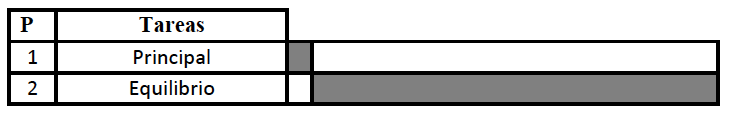
\includegraphics[scale=0.4]{./img/grafico3a.png}
 \caption{Funcionamiento práctica 3a.}
 \label{grafico3a}
\end{figure}

\subsection{Código del fichero practica3\_a.c}
\lstinputlisting{practicas/practica3a/practica_3a.c}

\subsection{Código del fichero practica3\_oil.c}
\lstinputlisting{practicas/practica3a/practica_3a.oil}

\subsection{Resultados}
Los niveles definidos para mantener el robot en equilibro han sido definidos para la superficie, en la que nosotros hemos utilizado el robot, puede producirse que en otro superficie se necesiten establecer otros niveles para mantener el robot en equilibrio.\\

A pesar de que sea resuelto el problema con el sensor de luz, el cual es muy sensible a los cambios de iluminación y la superficie en la que se ponga el robot, los resultados han sido buenos y se ha logrado mantener el robot en equilibrio durante un buen periodo de tiempo como se puede observar en el siguiente vídeo.\\

\textbf{Vídeo}: \url{http://www.youtube.com/watch?v=OFuzqQBd6Do} 